% [1,120,0,1 Cr3,13,32 Do0.1,2 Mp2,2 Cr3,13,32 Do0.1,2 Mp2,2 Cr3,9,64 Do0.1,2 Mp2,2 Cr3,9,64 Do0.1,2 S1(1x0)1,3 Lbx200 Do0.1,2 Lbx200 Do.1,2 Lbx200 Do]

\documentclass[tikz]{standalone}
\begin{document}
        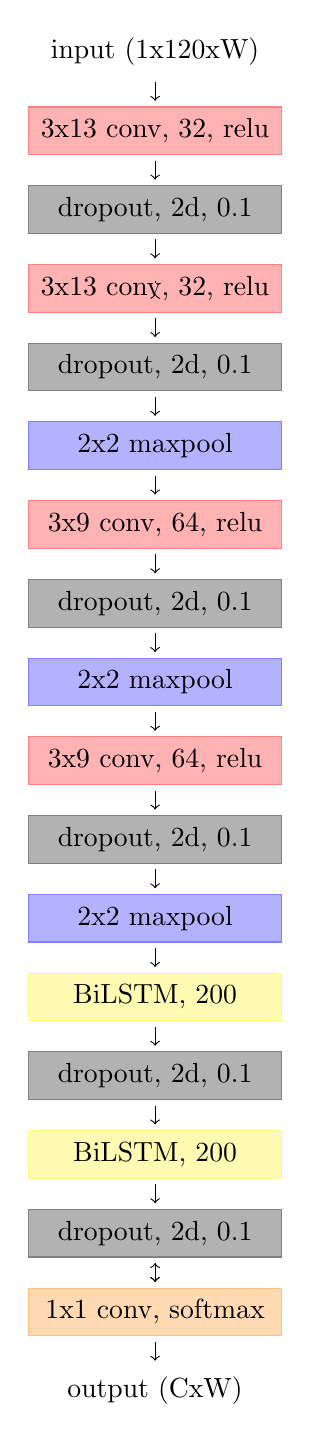
\begin{tikzpicture}[node distance = 1cm]
        \tikzset{
          base/.style={draw, align=center, minimum height=4ex, rectangle, text centered},
          proc/.style={base, draw=white, rectangle, text width=8.5em},
          conv/.style={proc, draw=red!50, fill=red!30},
          maxp/.style={proc, draw=blue!50, fill=blue!30},
          drop/.style={proc, draw=black!50, fill=black!30},
          lstm/.style={proc, draw=yellow!50, fill=yellow!30},
          soft/.style={proc, draw=orange!50, fill=orange!30},
          line/.style={draw, shorten <= 2pt, shorten >= 2pt, ->}
        }
        \node [proc] (input) {input (1x120xW)};
        \node [proc, conv, below of=input] (conv1) {3x13 conv, 32, relu};
        \node [proc, drop, below of=conv1] (drop1) {dropout, 2d, 0.1};
        \node [proc, maxp, below of=drop1] (maxp1) {2x2 maxpool};

	\node [proc, conv, below of=drop1] (conv2) {3x13 conv, 32, relu};
        \node [proc, drop, below of=conv2] (drop2) {dropout, 2d, 0.1};
        \node [proc, maxp, below of=drop2] (maxp2) {2x2 maxpool};

	\node [proc, conv, below of=maxp2] (conv3) {3x9 conv, 64, relu};
        \node [proc, drop, below of=conv3] (drop3) {dropout, 2d, 0.1};
        \node [proc, maxp, below of=drop3] (maxp3) {2x2 maxpool};

	\node [proc, conv, below of=maxp3] (conv4) {3x9 conv, 64, relu};
        \node [proc, drop, below of=conv4] (drop4) {dropout, 2d, 0.1};
        \node [proc, maxp, below of=drop4] (maxp4) {2x2 maxpool};

        \node [proc, lstm, below of=maxp4] (lstm1) {BiLSTM, 200};
        \node [proc, drop, below of=lstm1] (drop5) {dropout, 2d, 0.1};

        \node [proc, lstm, below of=drop5] (lstm2) {BiLSTM, 200};
        \node [proc, drop, below of=lstm2] (drop6) {dropout, 2d, 0.1};

        \node [proc, lstm, below of=drop6] (lstm3) {BiLSTM, 200};
        \node [proc, drop, below of=lstm2] (drop7) {dropout, 2d, 0.1};

        \node [proc, soft, below of=drop7] (softm) {1x1 conv, softmax};
        \node [proc, below of=softm] (output) {output (CxW)};

        \path [line] (input) -- (conv1);
        \path [line] (conv1) -- (drop1);
        \path [line] (drop1) -- (maxp1);
        \path [line] (maxp1) -- (conv2);
        \path [line] (conv2) -- (drop2);
        \path [line] (drop2) -- (maxp2);
	\path [line] (maxp2) -- (conv3);
        \path [line] (conv3) -- (drop3);
        \path [line] (drop3) -- (maxp3);
	\path [line] (maxp3) -- (conv4);
        \path [line] (conv4) -- (drop4);
        \path [line] (drop4) -- (maxp4);
	\path [line] (maxp4) -- (lstm1);
        \path [line] (lstm1) -- (drop5);
        \path [line] (drop5) -- (lstm2);
        \path [line] (lstm2) -- (drop6);
        \path [line] (drop6) -- (lstm3);
        \path [line] (lstm3) -- (drop7);
        \path [line] (drop7) -- (softm);
        \path [line] (softm) -- (output);
	\end{tikzpicture}
\end{document}
